%%% TO DO %%%
% implement siunitx package and change units

\documentclass[12pt]{article}

\usepackage{ishn}
\usetikzlibrary{decorations.markings}
\usetikzlibrary{patterns}
\usetikzlibrary{patterns.meta}
\usepackage{caption}
\usepackage{subcaption}

\makeindex[intoc]

\begin{document}
\robustify\dots
\sisetup{input-digits = 0123456789\dots}

\tikzset{middlearrow/.style={
        decoration={markings,
            mark= at position 0.5 with {\arrow{#1}} ,
        },
        postaction={decorate}
    }
}

\hypersetup{pageanchor=false}
\begin{titlepage}
	\begin{center}
		\vspace*{1em}
		\Huge
		\textbf{IB Electromagnetism}

		\vspace{1em}
		\large
		Ishan Nath, Lent 2023

		\vspace{1.5em}

		\Large

		Based on Lectures by Prof. Gordon Ogilvie

		\vspace{1em}

		\large
		\today
	\end{center}
	
\end{titlepage}
\hypersetup{pageanchor=true}

\tableofcontents

\newpage

\section{Introduction}
\label{sec:introduction}

\subsection{Charges and Currents}
\label{sub:charges_and_currents}

\emph{Electric charge}\index{electric charge} is a physical property of elementary particles. It is:
\begin{itemize}
	\item Positive, negative or zero.
	\item Quantized (an integer multiple of the \emph{elementary charge} $e$).
	\item Conserved (even if particles are created or destroyed).
\end{itemize}

By convention, the electron has charge $-e$, the proton has charge $+e$, and the neutron has charge $0$.

On macroscopic scales, the number of particles is so large that charge can be considered to have continuous \emph{electric charge density}\index{electric charge density} $\rho(\mathbf{x},t)$. The total charge in a volume $V$ is then
\[
Q = \int_{V} \rho \diff V
.\]

The \emph{electric current density}\index{electric charge density} $\mathbf{J}(\mathbf{x}, t)$ is the flux of electric charge per unit area. The current flowing through a surface $S$ is
\[
I = \int_{S} \mathbf{J} \cdot \diff \mathbf{S}
.\]

Consider a time-independent volume $V$ with boundary $S$. Since charge is conserved, we have
\begin{align*}
	\frac{\diff Q}{\diff t} &= -I, \\
	\frac{\diff}{\diff t} \int_{V} \rho \diff V + \int_{S} \mathbf{J} \cdot d \mathbf{S} &= 0, \\
	\int_{V} \biggl( \frac{\partial \rho}{\partial t} + \nabla \cdot \mathbf{J} \biggr) \diff V &= 0.
\end{align*}
Since this is true for any $V$, we must have
\[
\frac{\partial \rho}{\partial t} + \nabla \cdot \mathbf{J} = 0
.\]

This \emph{equation of charge conservation}\index{equation of charge conservation} has the typical form of a conservation law.

The discrete charge distribution of a single particle of charge $q_i$, and position vector $\mathbf{x}_i(t)$ is
\begin{align*}
	\rho &= q_i \delta( \mathbf{x} - \mathbf{x}_i(t)), \\
	\mathbf{J} &= q_i \mathbf{\dot x}_i \delta(\mathbf{x} - \mathbf{x}_i(t)).
\end{align*}
For $N$ particles, it is
\begin{align*}
	\rho &= \sum_{i = 1}^{N} q_i \delta(\mathbf{x} - \mathbf{x}_i(t)), \\
	\mathbf{J} &= \sum_{i = 1}^{N} q_i \mathbf{\dot x}_i \delta(\mathbf{x} - \mathbf{x}_i(t)).
\end{align*}
We can verify that these distributions satisfy the charge conservation equation.

\subsection{Fields and Forces}
\label{sub:fields_and_forces}

Electromagnetism is a \emph{field theory}\index{field theory}. Charged particles interact not directly, but by generating fields around them that are experienced by other charged particles.

In general, we have two time-dependent vector fields: the \emph{electric field}\index{electric field} $\mathbf{E}(\mathbf{x}, t)$, and the \emph{magnetic field}\index{magnetic field} $\mathbf{B}(\mathbf{x}, t)$.

The \emph{Lorentz force}\index{Lorentz force} on a particle of charge $q$ and velocity $\mathbf{v}$ is
\[
\mathbf{F} = q(\mathbf{E} + \mathbf{v} \times \mathbf{B})
.\]

\subsection{Maxwell's equations}
\label{sub:maxwells_equations}

In this course we will explore some consequences of \emph{Maxwell's equations}\index{Maxwell's equations}
\begin{align*}
	\nabla \cdot \mathbf{E} &= \frac{\rho}{\epsilon_0}, & \nabla \cdot \mathbf{B} &= 0, \\
	\nabla \times \mathbf{E} &= - \frac{\partial \mathbf{B}}{\partial t}, & \nabla \times \mathbf{B} &= \mu_0 \biggl( \mathbf{J} + \epsilon_0 \frac{\partial \mathbf{E}}{\partial t} \biggr).
\end{align*}
Some properties of Maxwell's equations are:
\begin{itemize}
	\item They are coupled linear PDE's in space and time.
	\item They involve two positive constants: $\epsilon_0$ (vacuum permittivity)\index{vacuum permittivity}, and $\mu_0$ (vacuum permeability)\index{vacuum permeability}.
	\item Charges $(\rho)$ and currents $(\mathbf{J})$ are the sources of the electromagnetic fields.
	\item Each equation has an equivalent integral form, related via the divergence theorem of Stokes' theorem.
	\item These are the vacuum equations that apply on microscopic scales (or in a vacuum). A related macroscopic version applies in media (for examples air).
	\item The equations are consistent with each other and with charge conservation. For example, $\nabla \cdot (M3) = \frac{\partial}{\partial t}(M2)$, and
		\[
		\frac{\partial \rho}{\partial t} + \nabla \cdot \mathbf{J} = \frac{\partial}{\partial t} (\epsilon_0 \nabla \cdot \mathbf{E}) + \nabla \cdot \biggl(- \epsilon_0 \frac{\partial \mathbf{E}}{\partial t} + \frac{1}{\mu_0} \nabla \times \mathbf{B} \biggr) = 0
		.\]
\end{itemize}

\subsection{Units}
\label{sub:units}

The SI unit of electric charge is the coulomb (\unit{\coulomb}). The elementary charge is (exactly)
\[
	e = \qty{1.602176634e-19}{\coulomb}
.\]
The SI unit of electric current is the ampere, or amp (\unit{\ampere}), equal to \qty{1}{\coulomb\per\second}.

The SI base units needed in electromagnetism are:
\begin{itemize}
	\item[] second (\unit{\second})
	\item[] metre (\unit{\metre})
	\item[] kilogram (\unit{\kilogram})
	\item[] ampere (\unit{\ampere})
\end{itemize}

From the Lorentz force law, we can see that the units of $\mathbf{E}$ and $\mathbf{B}$ must be
\begin{center}
	\unit{\kilogram\metre\per\second\cubed\per\ampere} and \unit{\kilogram\per\second\squared\per\ampere}.
\end{center}
The latter is also called the tesla (\unit{\tesla}). From Maxwell's equations, we can work out the units of $\epsilon_0$ and $\mu_0$. The experimentally determined values are
\begin{align*}
	\epsilon_0 &= \qty{8.854\dots e-12}{\per\kilogram\per\metre\cubed\second\tothe{4}\ampere\squared} \\
	\mu_0 &= \qty{1.256\dots e-6}{\kilogram\metre\per\second\squared\per\ampere\squared}\\
	      &\approx 4 \pi \times 10^{-7}\, \unit{\kilogram\metre\per\second\squared\per\ampere\squared}.
\end{align*}

The speed of light is (exactly)
\[
	c = \frac{1}{\sqrt{\mu_0 \eps_0}} = \qty{299792458}{\metre\per\second} \approx \qty{3e8}{\metre\per\second}
.\]

\newpage

\section{Electrostatics}
\label{sec:electrostatics}

In a time-independent situation, Maxwell's equations reduce to
\begin{align*}
	\nabla \cdot \mathbf{E} &= \frac{\rho}{\epsilon_0}, & \nabla \times \mathbf{E} &= \mathbf{0}, \\
	\nabla \cdot \mathbf{B} &= 0, & \nabla \times \mathbf{B} &= \mu_0 \mathbf{J}.
\end{align*}
Since $\mathbf{E}$ and $\mathbf{B}$ are decoupled, we can study them separately.

\emph{Electrostatics}\index{electrostatics} is the study of the electric field generated by a stationary charge distribution
\begin{align*}
	\nabla \cdot \mathbf{E} &= \frac{\rho}{\epsilon_0}, & \nabla \times \mathbf{E} &= \mathbf{0}.
\end{align*}

\subsection{Gauss' Law}
\label{sub:gauss_law}

Consider a closed surface $S$ enclosing a volume $V$. Integrating (M1) over $V$ and using the divergence theorem, we obtain \emph{Gauss' law}\index{Gauss' law}
\[
\int_{S} \mathbf{E} \cdot \diff \mathbf{S} = \frac{Q}{\epsilon_0}
,\]
where $Q = \int_{V} \rho \diff V$ is the total charge in $V$.

Gauss' law is the integral version of (M1) and is valid generally. This says that the electric flux of a closed surface is proportional to the total charge enclosed.

In special situations, we can use Gauss' law together with symmetry to deduce $\mathbf{E}$ from $\rho$. By choosing the \emph{Gaussian surface}\index{Gaussian surface} $S$ appropriately.

\subsubsection{Spherical Symmetry}
\label{subsub:spherical_symmetry}

Consider a spherically symmetric charge distribution, $\rho(r)$ in spherical polar coordinates, with total charge $Q$ contained within an outer radius $R$.

To have spherical symmetry, the electric field should have the form
\[
	\mathbf{E} = E(r) \mathbf{e}_r
.\]
This will satisfy (M3'), as required. To find $E(r)$, we apply Gauss' law to a sphere of radius $r$. If $r > R$, then
\[
\int_{S}\mathbf{E}\cdot \diff \mathbf{S} = E(r) \int_{S} \mathbf{e}_r \cdot \diff \mathbf{S} = E(r) \int_{S} \diff S = E(r) \, 4 \pi r^2 = \frac{Q}{\epsilon_0}
.\]
Thus, outside of the sphere of radius $R$,
\[
\mathbf{E} = \frac{Q}{4 \pi \epsilon_0 r^2}\mathbf{e}_r
.\]
So the external electric field of a spherically symmetric body depends only on the total charge.

The Lorentz force on a particle of charge $q$ in $r > R$ is
\[
\mathbf{F} = q \mathbf{E} = \frac{Qq}{4 \pi \epsilon_0 r^2} \mathbf{e}_r
.\]
This is the \emph{Coulomb force}\index{Coulomb force} between charged particles. The force is repulsive if the charges have the same sign $(Qq > 0)$ and attractive if they have opposite signs $(Qq < 0)$.

If we take the limit $R \to 0$, we obtain the electric field of a \emph{point charge}\index{point charge} $Q$, corresponding to
\[
\rho = Q \delta(\mathbf{x})
.\]

There is a close analogy between the Coulomb force and the gravitational force between massive particles,
\[
	\mathbf{F} = - \frac{GMm}{r^2} \mathbf{e}_r
.\]
Both involve an inverse-square law, and the product of the charges/masses. However,
\begin{itemize}
	\item While gravity is always attractive, electric forces can be repulsive or attractive.
	\item Gravity is very much weaker than the Coulomb force, e.g. for two protons the ratio of the electric to gravitational forces is
		\[
		\frac{e^2}{4 \pi \epsilon_0 G m_p^2} \approx 10^{36}
		.\]
		On the atomic scale, gravity is irrelevant. But positive and negative charges balance so accurately that on the planetary scale, gravity is dominant.
\end{itemize}

\subsubsection{Cylindrical Symmetry}
\label{subsub:cylindrical_symmetry}

Consider a cylindrically symmetric charge distribution $\rho(r)$ in cylindrical polar coordinates, with total charge $\lambda$ per unit length, contained within an outer radius $R$.

To have cylindrical symmetry,
\[
\mathbf{E} = E(r) \mathbf{e}_r
.\]
To find  $E(r)$ we apply Gauss' law to a cylinder of radius $r$ and arbitrary length $L$. Again, we consider $r > R$. Then, since only the curved part of the cylinder contributes to the flux,
\[
\int_{S}\mathbf{E} \cdot \diff \mathbf{S} = E(r) \int_{S}\mathbf{e}_r \cdot \diff \mathbf{S} = E(r) \int_{S} \diff S = E(r) 2 \pi r L = \frac{\lambda L}{\epsilon_0}
.\]
Thus, we get
\[
\mathbf{E} = \frac{\lambda}{2 \pi \epsilon_0 r} \mathbf{e_r}
.\]
In the limit $R \to 0$, we obtain the electric field of a \emph{line charge}\index{line charge} $\lambda$ per unit length, corresponding to
\[
\rho = \lambda \delta(x) \delta(y)
.\]

\subsubsection{Planar Symmetry}
\label{subsub:planar_symmetry}

We consider a planar charge distribution $\rho(z)$ in Cartesian coordinates, with total charge $\sigma$ per unit area, contained within a region $-d < z < d$ of thickness $2d$. We assume reflectional symmetry, so $\rho(z)$ is even.

To have planar symmetry, we need
\[
\mathbf{E} = E(z) \mathbf{e}_z
,\]
which will satisfy (M3'). Reflectional symmetry implies $E(-z) = -E(z)$. To find $E(z)$ for $z > 0$, apply Gauss' law to a ``Gaussian pillbox'' of height $2z$ and arbitrary area $A$. If $z > d$, then
\[
\int_{S}\mathbf{E} \cdot \diff \mathbf{S} = E(z)A - E(-z)A = 2E(z)A = \frac{\sigma A}{\epsilon_0}
.\]
Thus,
\[
\mathbf{E} =
\begin{cases}
	\frac{\sigma}{2 \epsilon_0} \mathbf{e}_z & z > d, \\
	-\frac{\sigma}{2 \epsilon_0} \mathbf{e}_z & $z < -d$.
\end{cases}
\]
In the limit $d \to 0$, we obtain the electric field of a \emph{surface charge}\index{surface charge} $\sigma$ per unit area, corresponding to
\[
\rho = \sigma \delta(z)
.\]

\subsubsection{Surface Charge and Discontinuity}
\label{subsub:surface_charge_and_discontinuity}

Let $\mathbf{n}$ be a unit vector normal to the charged surface, pointing from region 1 to region 2. In our example, $\mathbf{n} = \mathbf{e}_z$.

The discontinuity in $\mathbf{E}$ is given by
\[
	[\mathbf{n} \cdot \mathbf{E}] = \frac{\sigma}{\epsilon_0}
,\]
where $\sigma$ is the surface charge density, and
\[
	[X] = X_2 - X_1
\]
denotes a discontinuity. The tangential components are continuous (they are both 0), so
\[
	[\mathbf{n} \times \mathbf{E}] = \mathbf{0}
.\]

These equation apply to any surface charge (even if the surface is curved an non-uniform).

The first comes from applying Gauss' law to an infinitesimal Gaussian pillbox on the surface.

The second comes from considering an infinitesimal circuit that goes through the surface: in the limit, and by taking all orientations of loops, we can use Stokes' theorem to get the required result.

\subsection{The Electrostatic Potential}
\label{sub:the_electrostatic_potential}

For general $\rho(\mathbf{x})$, we cannot determine $\mathbf{E}(\mathbf{x})$ using Gauss' law alone.

Since $\nabla \times \mathbf{E} = \mathbf{0}$, we know that $\mathbf{E}$ can be written in terms of an \emph{electrostatic potential}\index{electrostatic potential} (or electric potential) $\Phi(\mathbf{x})$
\[
\mathbf{E} = - \nabla \Phi
.\]
The \emph{potential difference}\index{potential difference} (or \emph{voltage}\index{voltage}) between two points $\mathbf{x}_1$ and $\mathbf{x}_2$ is
\[
\Phi(\mathbf{x}_2) - \Phi(\mathbf{x}_1) = \int \diff \Phi = - \int_{\mathbf{x}_1}^{\mathbf{x}_2} \mathbf{E}(\mathbf{x}) \cdot \diff \mathbf{x}
,\]
and is path-independent because $\nabla \times \mathbf{E} = \mathbf{0}$.

The electric force on a particle of charge $q$ is
\[
\mathbf{F} = q \mathbf{E} = - q \nabla \Phi
\]
is a conservative force associated with the potential energy
\[
U(\mathbf{x}) = q \Phi(\mathbf{x})
.\]
(M1) implies that $\Phi$ satisfies \emph{Poisson's equation}
\[
- \nabla^2 \Phi = \frac{\rho}{\epsilon_0}
.\]
The solution can be written as an integral (over all space, assuming decay at infinity)
\[
\Phi(\mathbf{x}) = \frac{1}{4 \pi \epsilon_0} \int \frac{\rho(\mathbf{x}')}{|\mathbf{x} - \mathbf{x}'|} \Diff3 \mathbf{x}'
.\]
This is the convolution of $\rho(\mathbf{x})$ with the potential of a unit point charge $\frac{1}{4 \pi \epsilon_0 |\mathbf{x}|}$, which is the solution of
\[
- \nabla^2 \Phi = \frac{\delta (\mathbf{x})}{\epsilon_0}
,\]
satisfying $\Phi \to 0$ as $|\mathbf{x}| \to \infty$.

Note that $\mathbf{E}$ is unaffected if we add an arbitrary constant to $\Phi$. We usually choose this constant such that $\Phi \to 0$ as $|\mathbf{x}| \to \infty$. However if $\rho(\mathbf{x})$ does not decay sufficiently rapidly, this may not be possible. For example, a line charge has $E_r \propto \frac{1}{r}$, so $\Phi \propto \log r$, which does not decay.

\subsubsection{Point Charge}
\label{subsub:point_charge}

The potential due to a point charge $q$ at the origin is
\[
\Phi(\mathbf{x}) = \frac{q}{4 \pi \epsilon_0 |\mathbf{x}|} = \frac{q}{4 \pi \epsilon_0 r}
.\]

\subsubsection{Electric Dipole}
\label{subsub:electric_dipole}

This consists of two equal and opposite charge at difference positions. Without loss of generality, consider charges $-q$ at $\mathbf{x} = \mathbf{0}$ and $+q$ and $\mathbf{x} = \mathbf{d}$.

\begin{figure}[h]
	\centering
	\caption{Electric Dipole}
	\label{fig:electric_dipole}
	\vspace{1em}
	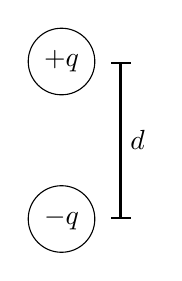
\begin{tikzpicture}
		\draw [|-|, thick](0,0) -- (0,2);
		\node [draw,circle] at (-0.75,2) {$+q$};
		\node [draw,circle] at (-0.75,0) {$-q$ };
		\node [right] at (0,1) {$d$};
	\end{tikzpicture}
\end{figure}

The potential due to the dipole will be
\[
\Phi(\mathbf{x}) = \frac{q}{4 \pi \epsilon_0} \biggl( - \frac{1}{|\mathbf{x}|} + \frac{1}{|\mathbf{x} - \mathbf{d}|} \biggr)
.\]
Applying Taylor's theorem to a scalar field, we get
\[
f(\mathbf{x} + \mathbf{h}) = f(\mathbf{x}) + (\mathbf{h} \cdot \nabla) f(\mathbf{x}) + \frac{1}{2} (\mathbf{h} \cdot \nabla)^2 f(\mathbf{x}) + \mathcal{O}(|\mathbf{h}|^3)
,\]
so applying this to our potential (and letting $|\mathbf{x}| = r$,)
\begin{align*}
	\Phi(\mathbf{x}) &= \frac{q}{4 \pi \epsilon_0} \biggl( -\frac{1}{r} + \frac{1}{r} - (\mathbf{d} \cdot \nabla) \frac{1}{r} + \mathcal{O}(|\mathbf{d}|^2)\biggr) \\
			 &= \frac{q}{4 \pi \epsilon_0} \frac{\mathbf{d} \cdot \mathbf{x}}{|\mathbf{x}|^3} + \mathcal{O}(|\mathbf{d}|^2).
\end{align*}
In the limit $|\mathbf{d}| \to 0$ with $q \mathbf{d}$ finite, we obtain a \emph{point dipole}\index{point dipole} with \emph{electric dipole moment}\index{electric dipole moment}
\[
\mathbf{p} = q \mathbf{d}
,\]
with potential
\[
\Phi(\mathbf{x}) = \frac{\mathbf{x} \cdot \mathbf{x}}{4 \pi \epsilon_0 |\mathbf{x}|^3}
.\]
The electric field can be found as
\[
\mathbf{E} = - \nabla \Phi = \frac{3(\mathbf{p} \cdot \mathbf{x})\mathbf{x} - |\mathbf{x}|^3 \mathbf{p}}{4 \pi \epsilon_0 |\mathbf{x}|^{5}}
.\]
In spherical polar coordinates aligned with $\mathbf{p}= p \mathbf{e}_z$,
\begin{align*}
	\Phi &= \frac{p \cos \theta}{4 \pi \epsilon_0 r^2}, \\
	E_r &= - \frac{\partial \Phi}{\partial r} = \frac{2 p \cos \theta}{4 \pi \epsilon_0 r^3}, \\
	E_\theta &= - \frac{1}{r} \frac{\partial \Phi}{\partial \theta} = \frac{p \sin \theta}{4 \pi \epsilon_0 r^3}, \\
	E_\phi &= 0.
\end{align*}
Note that
\begin{itemize}
	\item $\Phi$ and $\mathbf{E}$ are not spherically symmetric.
	\item They decrease more rapidly with $r$ than for a point charge.
\end{itemize}

A point dipole $\mathbf{p}$ at the origin corresponds to
\begin{align*}
	\rho(\mathbf{x}) &= - \mathbf{p} \cdot \nabla \delta(\mathbf{x}), \\
	\Phi(\mathbf{x}) &= \mathbf{p} \cdot \nabla \biggl( \frac{1}{4 \pi \epsilon_0 |\mathbf{x}|} \biggr).
\end{align*}

\subsubsection{Field Lines and Equipotentials}
\label{subsubsub:field_lines_and_equipotentials}

\emph{Electric field lines}\index{electric field lines} are the integral curves of $\mathbf{E}$, being tangent to $\mathbf{E}$ everywhere.

Since $\nabla \cdot \mathbf{E} = \frac{\rho}{\epsilon_0}$, the field lines begin at positive charges and end on negative charges.

Furthermore, in electrostatics $\mathbf{E} = - \nabla \Phi$, so the field lines are perpendicular to the equipotential surface $\Phi = \rm{constant}$.


\begin{figure}[h]
	\centering
	\caption{Electric Field Lines}
	\label{fig:electric_field_lines}
	\begin{subfigure}{0.5\textwidth}
		\centering
	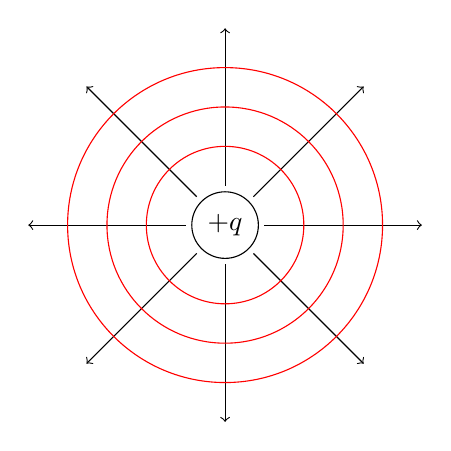
\begin{tikzpicture}
		\node [draw,circle] at (0,0) {$+q$};
		\draw [->](0,0.5) -- +(0,2);
		\draw [->](0.36,0.36) -- +(1.4,1.4);
		\draw [->](0.5,0) -- +(2,0);
		\draw [->](0.36,-0.36) -- +(1.4,-1.4);
		\draw [->](0,-0.5) -- +(0,-2);
		\draw [->](-0.36,-0.36) -- +(-1.4,-1.4);
		\draw [->](-0.5,0) -- +(-2,0);
		\draw [->](-0.36,0.36) -- +(-1.4,1.4);
		\draw [red] (0,0) circle (1);
		\draw [red] (0,0) circle (1.5);
		\draw [red] (0,0) circle (2);
	\end{tikzpicture}
	\caption{Point charge}
	\end{subfigure}%
	\begin{subfigure}{0.5\textwidth}
		\centering
	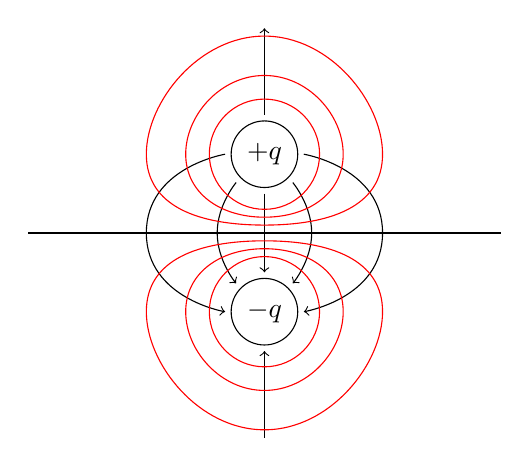
\begin{tikzpicture}
		\node [draw,circle] at (0,1) {$+q$};
		\node [draw,circle] at (0,-1) {$-q$};
		\draw (-3,0) -- (3,0);
		\draw [->] (0,0.5) -- +(0,-1);
		\draw [->] plot [smooth, tension = 1] coordinates {(-0.36,0.64) (-0.6, 0) (-0.36, -0.64)};
		\draw [->] plot [smooth, tension = 1] coordinates {(0.36,0.64) (0.6, 0) (0.36, -0.64)};
		\draw [->] plot [smooth, tension = 1.5] coordinates {(-0.5,1) (-1.5, 0) (-0.5, -1)};
		\draw [->] plot [smooth, tension = 1.5] coordinates {(0.5,1) (1.5, 0) (0.5, -1)};
		\draw [->] (0,1.5) -- +(0,1.1);
		\draw [<-] (0,-1.5) -- +(0,-1.1);
		\draw [red] (0,1) circle (0.7);
		\draw [red] (0,-1) circle (0.7);
		\draw [red] plot [smooth cycle, tension = 1] coordinates {(0,0.2) (1, 1) (0,2) (-1,1)};
		\draw [red] plot [smooth cycle, tension = 1] coordinates {(0,-0.2) (1, -1) (0,-2) (-1,-1)};
		\draw [red] plot [smooth cycle, tension = 1] coordinates {(0,0.1) (1.5, 1) (0,2.5) (-1.5,1)};
		\draw [red] plot [smooth cycle, tension = 1] coordinates {(0,-0.1) (1.5,-1) (0,-2.5) (-1.5,-1)};
	\end{tikzpicture}
	\caption{Dipole}
	\end{subfigure}
\end{figure}

\subsubsection{Dipole in an External Field}
\label{subsub:dipole_in_an_external_field}

Consider a dipole $\mathbf{p}$ in an external electric field $\mathbf{E} = - \nabla \Phi$ generated by distinct charges. If the dipole has charge $-q$ at $\mathbf{x}$ and $+q$ at $\mathbf{x} + \mathbf{d}$, then the potential energy of the dipole due to the external field is
\[
U = -q \Phi(\mathbf{x}) + q \Phi(\mathbf{x} + \mathbf{d}) = q (\mathbf{d} \cdot \nabla) \Phi(\mathbf{x}) + \mathcal{O}(|\mathbf{d}|^2)
.\]
In the limit of a point dipole,
\[
U = \mathbf{p} \cdot \nabla \Phi = - \mathbf{p} \cdot \mathbf{E}
.\]
This is minimized when $\mathbf{p}$ is aligned with $\mathbf{E}$.

\subsubsection{Multipole Expansion}
\label{subsub:multipole_expansion}

For a general charge distribution $\rho(\mathbf{x})$ confined to a ball $\{V \mid |\mathbf{x}| < \ell\}$, then
\[
\Phi(\mathbf{x}) = \frac{1}{4 \pi \epsilon_0} \int_{V} \frac{\rho(\mathbf{x}')}{|\mathbf{x} - \mathbf{x}'|} \Diff3 \mathbf{x}'
.\]
For an external potential with $|\mathbf{x}| > R$, we can expand
\begin{align*}
	\frac{1}{|\mathbf{x} - \mathbf{x}'|} &= \frac{1}{r} - (\mathbf{x}' \cdot \nabla) \frac{1}{r} + \frac{1}{2} (\mathbf{x}' \cdot \nabla)^2 \frac{1}{r} + \mathcal{O}(|\mathbf{x}'|^3) \\
					     &= \frac{1}{r} \biggl[ 1 + \frac{\mathbf{x}' \cdot \mathbf{x}}{r^2} + \frac{3(\mathbf{x}' \cdot \mathbf{x})^2 - |\mathbf{x}'|^2|\mathbf{x}|^2}{2r^{4}} + \mathcal{O} \biggl( \frac{R^3}{r^3} \biggr) \biggr].
\end{align*}
This leads to the \emph{multipole expansion}\index{multipole expansion} of the potential
\[
\Phi(\mathbf{x}) = \frac{1}{4 \pi \epsilon_0} \biggl( \frac{Q}{r} + \frac{\mathbf{p} \cdot \mathbf{x}}{r^3} + \frac{1}{2} \frac{Q_{ij}x_ix_j}{r^{5}} + \cdots \biggr)
.\]
The first three multipole moments are the:
\begin{itemize}
	\item total charge (or monopole moment)\index{monopole moment} - a scalar, where
		\[
			Q = \int_{V} \rho(\mathbf{x}) \Diff3 \mathbf{x}.
		\]
	\item electric dipole moment - a vector, where
		\[
			\mathbf{p} = \int_{V} \mathbf{x} \rho(\mathbf{x}) \Diff3 \mathbf{x}.
		\]
	\item electric quadrupole moment - a traceless, symmetric second order tensor
		\[
			Q_{ij} = \int_{V}(3x_ix_j - |\mathbf{x}|^2 \delta_{ij}) \rho(\mathbf{x}) \Diff3 \mathbf{x}
		\]
\end{itemize}

For $r \gg R$, $\Phi$ and $\mathbf{E}$ look increasingly like those of a point charge $Q$ unless $Q = 0$, in which case they look like those of a point dipole, unless $\mathbf{p} = 0$, etc.

\subsection{Electrostatic Energy}
\label{sub:electrostatic_energy}\index{electrostatic energy}

The work done against the electric force $\mathbf{F} = q \mathbf{E}$ in bringing a particle of charge $q$ from infinity (where we assume $\Phi = 0$) to $\mathbf{x}$ is
\[
- \int_{\infty}^{\mathbf{x}} \mathbf{F} \cdot \diff \mathbf{x} = +q \int_{\infty}^{\mathbf{x}} \nabla \Phi \cdot \diff \mathbf{x} = q \Phi (\mathbf{x})
.\]

Consider assembling a configuration of $N$ point charges one by one. Particle $i$ of charge $q_i$ is brought from $\infty$ to $\mathbf{x}_i$, while the previous particles remain fixed.
\begin{enumerate}[label = Particle \arabic*.]
	\item There is no work involved, so $W_1 = 0$.
	\item
		\[
		W_1 = q_2 \biggl( \frac{q}{4 \pi \epsilon_0 |\mathbf{x}_2 - \mathbf{x}_1|} \biggr)
		.\]
	\item
		\[
		W_3 = q_3 \biggl( \frac{q_1}{4 \pi \epsilon_0 |\mathbf{x}_3 - \mathbf{x}_1|} + \frac{q_2}{4 \pi \epsilon_0|\mathbf{x}_3 - \mathbf{x}_2|} \biggr)
		,\]
\end{enumerate}
and so on. The total work done is
\[
U = \sum_{i = 1}^{N} W_i = \sum_{i = 2}^{N} \sum_{j = 1}^{i-1} \frac{q_i q_j}{4 \pi \epsilon_0 |\mathbf{x}_i - \mathbf{x}_j|}
.\] 
This can be rewritten as
\[
	U = \frac{1}{2} \sum_{i = 1}^{N}\sum_{\substack{j=1\\j\neq i}}^{N} \frac{q_i q_j}{4 \pi \epsilon_0|\mathbf{x}_i - \mathbf{x}_j|}
,\]
or
\[
U = \frac{1}{2} \sum_{i = 1}^{N} q_i \Phi(\mathbf{x}_i)
.\]

Generalizing to a continuous charge distribution $\rho(\mathbf{x})$, occupying a finite volume $V$,
\[
U = \frac{1}{2} \int_{V} \rho(\mathbf{x}) \Phi(\mathbf{x}) \Diff3 \mathbf{x} = \frac{1}{2} \int_{V} \rho \Phi \diff V
.\]
Using (M1) we have
\begin{align*}
	U &= \frac{1}{2} \int_{V} (\epsilon_0 \nabla \cdot \mathbf{E}) \Phi \diff V = \frac{\epsilon_0}{2} \int_{V} (\nabla \cdot (\Phi \mathbf{E}) - \mathbf{E} \cdot \nabla \Phi) \diff V \\
	  &= \frac{\epsilon_0}{2} \int_{S} \phi \mathbf{E} \cdot \diff \mathbf{S} + \int_{V} \frac{\epsilon_0|\mathbf{E}|^2}{2} \diff V
.\end{align*}

Let $S = \partial V$ be a sphere of radius $R \to \infty$. Then $\Phi = \mathcal{O}(R^{-1})$, and $\mathbf{E} = \mathcal{O}(R^{-2})$ on $S$, while the area of $S$ is $\mathcal{O}(R^2)$, so the area integral is $\mathcal{O}(R^{-1})$ and goes to zero as $R \to \infty$. Thus,
\[
U = \int \frac{\epsilon_0 |\mathbf{E}|^2}{2} \diff V
,\]
integrated over all space.

This implies that energy is stored in the electric field, even in a vacuum.

Any of the expression for $U$ suggest that the self-energy of a point charge is infinite. We can discard this as it is unchanging and causes no force.

\subsection{Conductors}
\label{sub:conductors}

In an \emph{conductor}\index{conductor} such as a metal, some charges (usually electrons) can move freely. In electrostatics we require
\[
	\mathbf{E} = \mathbf{0}, \qquad \Phi = \rm{constant}
\]
inside a conductor, hence $\rho = 0$. Otherwise free charges would move in response to the electric force and a current would flow.

A surface charge density $\rho$ can exist on the surface of a conductor, which is an equipotential.

Taking a normal $\mathbf{n}$ to the point of the conductor, the condition
\[
	[\mathbf{n} \cdot \mathbf{E}] = \frac{\sigma}{\epsilon_0} \implies \mathbf{n} \cdot \mathbf{E} = \frac{\sigma}{\epsilon_0}
\]
immediately outside the conductor.

The constant potential of a conductor can be set by connecting it to a battery or another conductor. An \emph{earthed} (or \emph{grounded}) conductor is connected to the ground, usually taken as $\Phi = 0$.

To find $\Phi(\mathbf{x})$ and $\mathbf{E}(\mathbf{x})$ due to a charge distribution $\rho(\mathbf{x})$ in the presence of conductors with surfaces $S_i$ and potentials $\Phi_i$, we solve Poisson's equation
\[
- \nabla^2 \Phi = \frac{\rho}{\epsilon_0}
,\]
with Dirichlet boundary conditions $\Phi = \Phi_i$ on $S_i$. The solution depends linearly on $\rho$ and $\{\Phi_i\}$.

\begin{exbox}
	Consider a point charge $q$ at position $(0,0,h)$ in a half-space $z > 0$, bounded by an earthed conducting wall ($\Phi = 0$ on $z = 0$).

	By the method of images, the solution in $z > 0$, is identical to that of a dipole, with image charge $-q$ at $(0, 0, -h)$.

	This is as the wall coincides with an equipotential of the dipole. The induced surface charge density on the wall can be worked out from
	\[
	\frac{\sigma}{\epsilon_0} = \mathbf{n} \cdot \mathbf{E} = E_z = - \frac{qh}{4 \pi \epsilon_0 (r^2 + h^2)^{3/2}}
	,\]
	where $r = \sqrt{x^2 + y^2}$. The total induced surface charge is
	\[
	\int_{0}^{\infty} \sigma 2 \pi r \diff r = - q h \int_{0}^{\infty} \frac{r \diff r}{(r^2 + h^2)^{3/2}} = -q
	.\]
\end{exbox}

\begin{figure}[h]
	\centering
	\caption{Point Charge and Wall}
	\label{fig:point_charge_and_wall}
	\begin{tikzpicture}
		\draw[fill] (0,2) circle (0.05);
		\draw[fill] (0,-2) circle (0.05);
		\draw (-5,0) -- (5,0);
		\draw[<->] (0,0.1) -- (0,1.85);
		\draw[<->] (0,-0.1) -- (0,-1.85);
		\node[right] at (0,1) {$h$};
		\node[right] at (0,-1) {$h$};
		\node[right] at (0,2) {$+q$};
		\node[right] at (0,-2) {$-q$};
		\draw (0.15, 1.85) -- (1.85,0.1);
		\node[below] at (0.925,0) {$r$};
		\draw[->] (2.5,0.1) -- (2.5,0.8);
		\node[above] at (2.5,0.8) {\small$z>0$};
		\node[right] at (5,0) {\small$z=0$};
	\end{tikzpicture}
\end{figure}

A simple \emph{capacitor}\index{capacitor} consists of two separated conductors carrying charges $\pm Q$.

If the potential difference (voltage) between them is $V$, then the capacitance\index{capacitance} is defined by
\[
C = \frac{Q}{V}
,\]
and depends only on the geometry, because $\Phi$ depends linearly on $Q$.

\begin{exbox}
	Consider two infinite parallel plates separated by $d$. Let the plate surfaces be at $z = 0$, $z = d$, and have surface charge densities $\pm \sigma$. Then, $\mathbf{E} = E \mathbf{e}_z$ with $E = \sigma/\epsilon_0$ constant for $0 < z < d$.

	Then $\Phi = - Ez + \rm{constant}$ and $V = Ed$.

	The same solution holds approximately for parallel plates of area $A \gg d^2$ if end-effects are neglected. So,
	\[
	C = \frac{Q}{V} \approx \frac{\sigma A}{E d} \approx \frac{\epsilon_0 A}{d}
	.\]
	The electrostatic energy stored in the capacitor is
	\[
	U = \int \frac{\epsilon_0 |\mathbf{E}|^2}{2} \diff V \approx \frac{\epsilon_0 E^2}{2} A d \approx \frac{1}{2} CV^2
	.\]
	In general,
	\[
	U = \frac{1}{2} CV^2 = \frac{Q^2}{2C}
	.\]
	The work done in moving an element of charge $\delta Q$ from one plate to another is $\delta W = V \delta Q$. So the total work done is
	\[
	\int_{0}^{Q} \frac{Q'}{C} \diff Q' = \frac{Q^2}{2C}
	.\]
	Or we can use
	\[
	U = \frac{1}{2} \int \rho \Phi \diff V = \frac{1}{2} Q \Phi_{+} - \frac{1}{2} Q \Phi_{-} = \frac{1}{2} Q V
	.\]
\end{exbox}

\begin{figure}[h]
	\centering
	\caption{Capacitors}
	\label{fig:capacitors}
	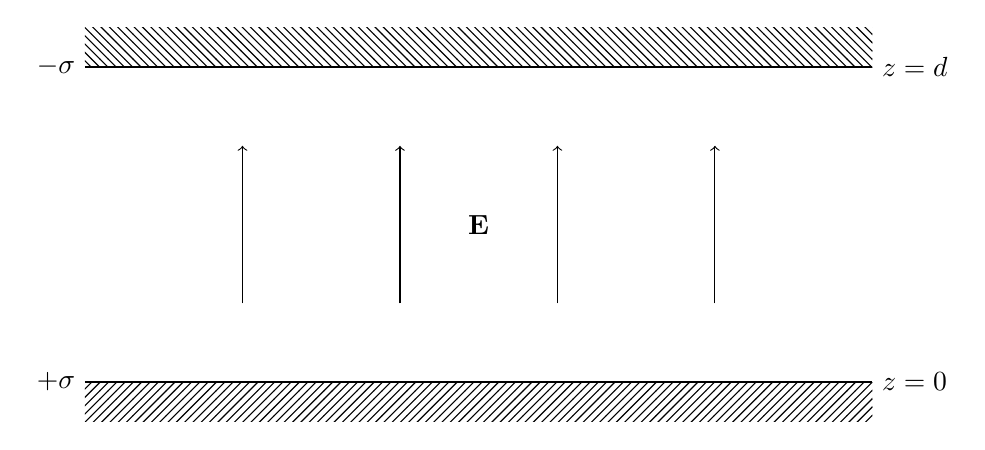
\begin{tikzpicture}
		\draw (-5, -2) -- (5, -2);
		\draw (-5, 2) -- (5, 2);
		\draw[->] (-3, -1) -- (-3, 1);
		\draw[->] (-1, -1) -- (-1, 1);
		\draw[->] (1, -1) -- (1, 1);
		\draw[->] (3, -1) -- (3, 1);
		\node[left] at (-5,-2) {$+\sigma$};
		\node[left] at (-5,2) {$-\sigma$};
		\node[right] at (5,-2) {$z=0$};
		\node[right] at (5,2) {$z=d$};
		\fill[pattern = north west lines] (-5,2) rectangle +(10,0.5);
		\fill[pattern = north east lines] (-5,-2) rectangle +(10,-0.5);
		\node at (0,0) {$\mathbf{E}$};
	\end{tikzpicture}
\end{figure}

\newpage

\section{Magnetostatics}
\label{sec:magnetostatics}

\emph{Magnetostatics}\index{magnetostatics} is the study of the magnetic field generated by a stationary current distribution:
\begin{align*}
	\nabla \times \mathbf{B} &= \mu_0 \mathbf{J} \tag{M4'}\label{eq:m4'}\\
	\nabla \cdot \mathbf{B} &= 0 \tag{M2}\label{eq:m2}
\end{align*}

From (\ref{eq:m4'}), we get $\nabla \cdot \mathbf{J} = 0$, the time-independent equation of charge conservation.

\subsection{Amp\`{e}re's Law}
\label{sub:amperes_law}

Consider a closed curve $C$ that is the boundary of an open surface $S$. Integrate (\ref{eq:m4'}) over $S$ and applying Stokes' theorem, we obtain \emph{Amp\`{e}re's law}\index{Amp\`{e}re's law}
\[
\int_{C} \mathbf{B} \cdot \diff \mathbf{x} = \mu_0 I
,\]
where
\[
I = \int_{S} \mathbf{J} \cdot \diff \mathbf{S}
\]
is the total current through $S$.

Since $\nabla \cdot \mathbf{J} = 0$, the same current $I$ flows through any open surface $S$ such that $\partial S = C$.

Amp\`{e}re's law is the integral version of (\ref{eq:m4'}) and is valid provided $\mathbf{E}$ is constant through time. In words, it says:
\begin{center}
	The circulation of magnetic field around a loop is proportional to the total current through the loop.
\end{center}

In special situations, we can use Amp\`{e}re's law, together with symmetry to deduce $\mathbf{B}$ from $\mathbf{J}$.

A cylindrically symmetric situation could involve:
\begin{itemize}
	\item An axial current distribution $J_z(r)\mathbf{e}_z$,
	\item An azimuthal current distribution $J_{\phi}(r)\mathbf{e}_{\phi}$,
\end{itemize}
or a combination. Since $\nabla \cdot \mathbf{J} = 0$, we have no radial component.

The same applies to $\mathbf{B}$. Hence the curl in Maxwell's equations implies $B_{\phi}$ is linearly related to $J_z$, and $B_z$ is linearly related to $J_{\phi}$.

\subsubsection{Long Straight Wire}
\label{subsub:long_straight_wire}

A cylindrical wire of radius $R$ carries a total current $I$ parallel to its axis.

To find $B_{\phi}(r)$ generated by $J_z(r)$, we apply Amp\`{e}re's law to a circle $C$ of radius $r$. Here $S$ is a disc.

\begin{figure}[h]
	\centering
	\caption{Long Straight Wire}
	\label{fig:long_straight_wire}
	\begin{tikzpicture}
		\draw (-1, -3) -- (-1, 3);
		\draw (1, -3) -- (1, 3);
		\draw (0,3) circle (1 and 0.3);
		\draw (-1,-3) arc (180:360:1 and 0.3);
		\draw[red] (-1,1) arc (113.5:426.5:2.5 and 0.75);
		\draw (0,3) -- (0.5,3.253);
		\node[below] at (0.5, 3.253) {\small $R$};
		\draw[->] (0,1.7) -- (0, 2.1);
		\node at (0, 2.3) {\small $\mathbf{I}$};
		\draw[red] (0,0.35) -- (1.5,0.92);
		\node[red] at (0.5, 0.3) {\small $r$};
		\node[red] at (-0.5, 0.35) {\small $S$};
	\end{tikzpicture}
\end{figure}

If $r > R$, then
\begin{align*}
	\int_{C} \mathbf{B} \cdot \diff \mathbf{x} &+ B_{\phi}(r) \int_{C} \mathbf{e}_{\phi} \cdot \diff \mathbf{x} = B_{\phi}(r) \int_{C} \diff \ell \\
						   &= B_{\phi}(r) 2 \pi r = \mu_0 I.
\end{align*}

Therefore, outside the wire,
\[
\mathbf{B} = \frac{\mu_0 I}{2 \pi r} \mathbf{e}_{\phi}
.\]

\subsubsection{Solenoid}
\label{subsub:solenoid}

A thin wire is coiled arund a cylindrical tube of radius $R$. An \emph{ideal solenoid}\index{ideal solenoid} is infinitely long and tightly wound, having cylindrical geometry and purely azimuthal current.

The wire carries current $I$ and has $N$ turns per unit length of the tube.

\begin{figure}[h]
	\centering
	\caption{Solenoid}
	\label{fig:solenoid}
	\begin{tikzpicture}
		\draw (-1, -3) -- (-1, 3);
		\draw (1, -3) -- (1, 3);
		\draw (0,3) circle (1 and 0.3);
		\draw (-1,-3) arc (180:360:1 and 0.3);
		\draw (0,3) -- (0.5,3.253);
		\node[below] at (0.5, 3.253) {\small $R$};
		\draw[blue,middlearrow={>}] (-1,-2.2) to[out=170,in=-10] (1,-1.9);
		\draw[blue,middlearrow={>}] (-1,-2) to[out=170,in=-10] (1,-1.7);
		\draw[blue,middlearrow={>}] (-1,-1.8) to[out=170,in=-10] (1,-1.5);
		\draw[blue,middlearrow={>}] (-1,-1.6) to[out=170,in=-10] (1,-1.3);
		\draw[blue,middlearrow={>}] (-1,-1.4) to[out=170,in=-10] (1,-1.1);
		\draw[blue,middlearrow={>}] (-1,-1.2) to[out=170,in=-10] (1,-0.9);
		\draw[blue,middlearrow={>}] (-1,-1) to[out=170,in=-10] (1,-0.7);
		\draw[red,middlearrow={>}] (0.7, -1.9) -- (0.7,-0.9);
		\draw[red,middlearrow={>}] (0.7, -0.9) -- (1.7,-0.9);
		\draw[red,middlearrow={>}] (1.7,-0.9) -- (1.7,-1.9);
		\draw[red,middlearrow={>}] (1.7,-1.9) -- (0.7,-1.9);
		\node[red] at (1.4, -1.4) {\small $S$};
		\node[red] at (1.4,-0.7) {\small $C$};
		\draw[red,|-|] (0,-0.6) -- (0.7,-0.6);
		\node[red,above] at (0.35,-0.6) {$a$};
		\draw[red,|-|] (0, -0.1) -- (1.7, -0.1);
		\node[red,above] at (0.85,-0.1) {$b$};
		\draw[red,|-|] (2,-1.9) -- (2,-0.9);
		\node[red,right] at (2,-1.45) {$L$};
	\end{tikzpicture}
\end{figure}

To find $B_z(r)$ generated by $J_{\phi}(r)$, we apply Amp\`{e}re's law to a rectangular loop $C$. Taking $a < b < R$ or $R < a < b$ gives
\[
L(B_z(a) - B_z(b)) = 0
.\]
Taking $a < R < b$ gives
\[
L(B_z(a) - B_z(b)) = \mu_0 N L I
.\]
Assuming that $B_z(r) \to 0$ as $r \to \infty$, we deduce that
\[
B_z(r) =
\begin{cases}
	\mu_0 N I & r < R,\\
	0 & r > R.
\end{cases}
\]

The ideal solenoid is an example of a \emph{surface current}\index{surface current}. Here it is of the form
\[
J_{\phi}(r) = K_{\phi}\delta(r - R),
.\]
where $K_{\phi} = NI$. Generally, a \emph{surface current density}\index{surface current density} $\mathbf{K}$ produces a discontinuity in the tangential magnetic field:
\[
	[\mathbf{n} \times \mathbf{B}] = \mu_0 \mathbf{K}
.\]
This follows from Ampere's law applied to a loop through a surface, where we take $L, h \to 0$.

\begin{figure}[h]
	\centering
	\caption{Surface Current}
	\label{fig:surface_current}
	\begin{tikzpicture}
		\draw (-7,0) -- (1,-1) -- (7,1) -- (-1,2) -- cycle;
		\draw[red] (0,0) -- (0,0.2) -- (1,0.5333) -- (1,0.3333);
		\draw[red,dashed] (1,0.3333) -- (1,0) -- (0,-0.3333) -- (0,0);
		\draw[->] (4, 0.5) -- (4,0.9);
		\node[above] at (4,0.9) {\small $\mathbf{n}$};
		\draw[red,|-|] (0,0.5) -- (1,0.8333);
		\node[red,above] at (0.5,0.7) {\small $L$};
		\draw[red,|-|] (1.2,0.6333) -- (1.2,0.3);
		\node[red,right] at (1.2,0.5) {\small $h$};
	\end{tikzpicture}
\end{figure}

Applying the same reasoning with (\ref{eq:m2}), we get
\[
	[\mathbf{n} \cdot \mathbf{B}] = 0
,\]
so the normal component is continuous.

\subsection{Magnetic Vector Potential}
\label{sub:magnetic_vector_potential}

(\ref{eq:m2}) implies that $\mathbf{B}$ can be written in terms of a \emph{magnetic vector potential}\index{magnetic vector potential} $\mathbf{A}(\mathbf{x})$:
\[
\mathbf{B} = \nabla \times \mathbf{A}
.\]
$\mathbf{A}$ is not unique. If we make a \emph{gauge transformation}\index{gauge transformation}, replacing $\mathbf{A}$ with
\[
\mathbf{A}' = \mathbf{A} + \nabla \chi
,\]
where $\chi(\mathbf{x})$ is an arbitrary scalar field, then $\mathbf{B}$ is unchanged, as
\[
\mathbf{B} = \nabla \times \mathbf{A} = \nabla \times \mathbf{A}'
.\]
A convenient gauge for many calculation is the \emph{Coulomb gauge}\index{Coulomb gauge} in which $\nabla \cdot \mathbf{A} = 0$.

We can assume this condition without loss of generality. If $\nabla \cdot \mathbf{A} \neq 0$, then we can make a gauge transformation $\nabla \cdot \mathbf{A}' = 0$ by choosing $\chi$ to be the solution of Poisson's equation
\[
- \nabla^2 \chi = \nabla \cdot \mathbf{A}
.\]
In terms of $\mathbf{A}$, (\ref{eq:m4'}) becomes
\[
\nabla \times (\nabla \times \mathbf{A}) = \mu_0 \mathbf{J}
.\]
Using the identity
\[
	\nabla \times (\nabla \times \mathbf{A}) = \nabla (\nabla \cdot \mathbf{A}) - \nabla^2 \mathbf{A}
,\]
and assuming a Coulomb gauge, we obtain Poisson's equation in vector form:
\[
- \nabla^2 \mathbf{A} = \mu_0 \mathbf{J}
.\]

\subsection{The Biot-Savart Law}
\label{sub:the_biot_savart_law}

The solution of Poisson's equation is
\[
\mathbf{A}(\mathbf{x}) = \frac{\mu_0}{4 \pi} \int \frac{\mathbf{J}(\mathbf{x}')}{|\mathbf{x} - \mathbf{x}'|} \Diff3 \mathbf{x}'
.\]
We should check that the solution satisfies the assumed Coulomb gauge condition:
\begin{align*}
	\nabla \cdot \mathbf{A}(\mathbf{x}) &= \frac{\mu_0}{4 \pi} \int_{V} \nabla \cdot \biggl( \frac{\mathbf{J}(\mathbf{x}')}{|\mathbf{x} - \mathbf{x}'|} \biggr) \Diff3 \mathbf{x}' \\
					    &= \frac{\mu_0}{4 \pi} \int_{V} \mathbf{J}(\mathbf{x}') \cdot \nabla \biggl( \frac{1}{|\mathbf{x} - \mathbf{x}'|} \biggr) \Diff3 \mathbf{x}' \\
					    &= - \frac{\mu_0}{4 \pi} \int_{V} \mathbf{J}(\mathbf{x}') \cdot \nabla' \biggl( \frac{1}{|\mathbf{x} - \mathbf{x}'|} \biggr) \Diff3 \mathbf{x}' \\
					    &= - \frac{\mu_0}{4 \pi} \int_{V} \nabla' \cdot \biggl( \frac{\mathbf{J}(\mathbf{x}')}{|\mathbf{x} - \mathbf{x}'|} \biggr) \Diff3 \mathbf{x}' \\
					    &= - \frac{\mu_0}{4 \pi} \int_{\partial V} \frac{\mathbf{J}(\mathbf{x}') \cdot \diff \mathbf{S}'}{|\mathbf{x} - \mathbf{x}'|}.
\end{align*}
This is $0$, as assumed, if the current is contained in some finite volume and we take $V$ to be at least as large, or if $\mathbf{J}$ decays sufficiently as $|\mathbf{x}| \to \infty$.

\newpage

\printindex

\end{document}
